\begin{figure}[h!]
    \centering
    \caption{Estimates of the share pocketed by landlords by the relative 
             change in workplace MW to change in residence MW, urban ZIP codes}
    \label{fig:rho_by_decile_MW_gap}

	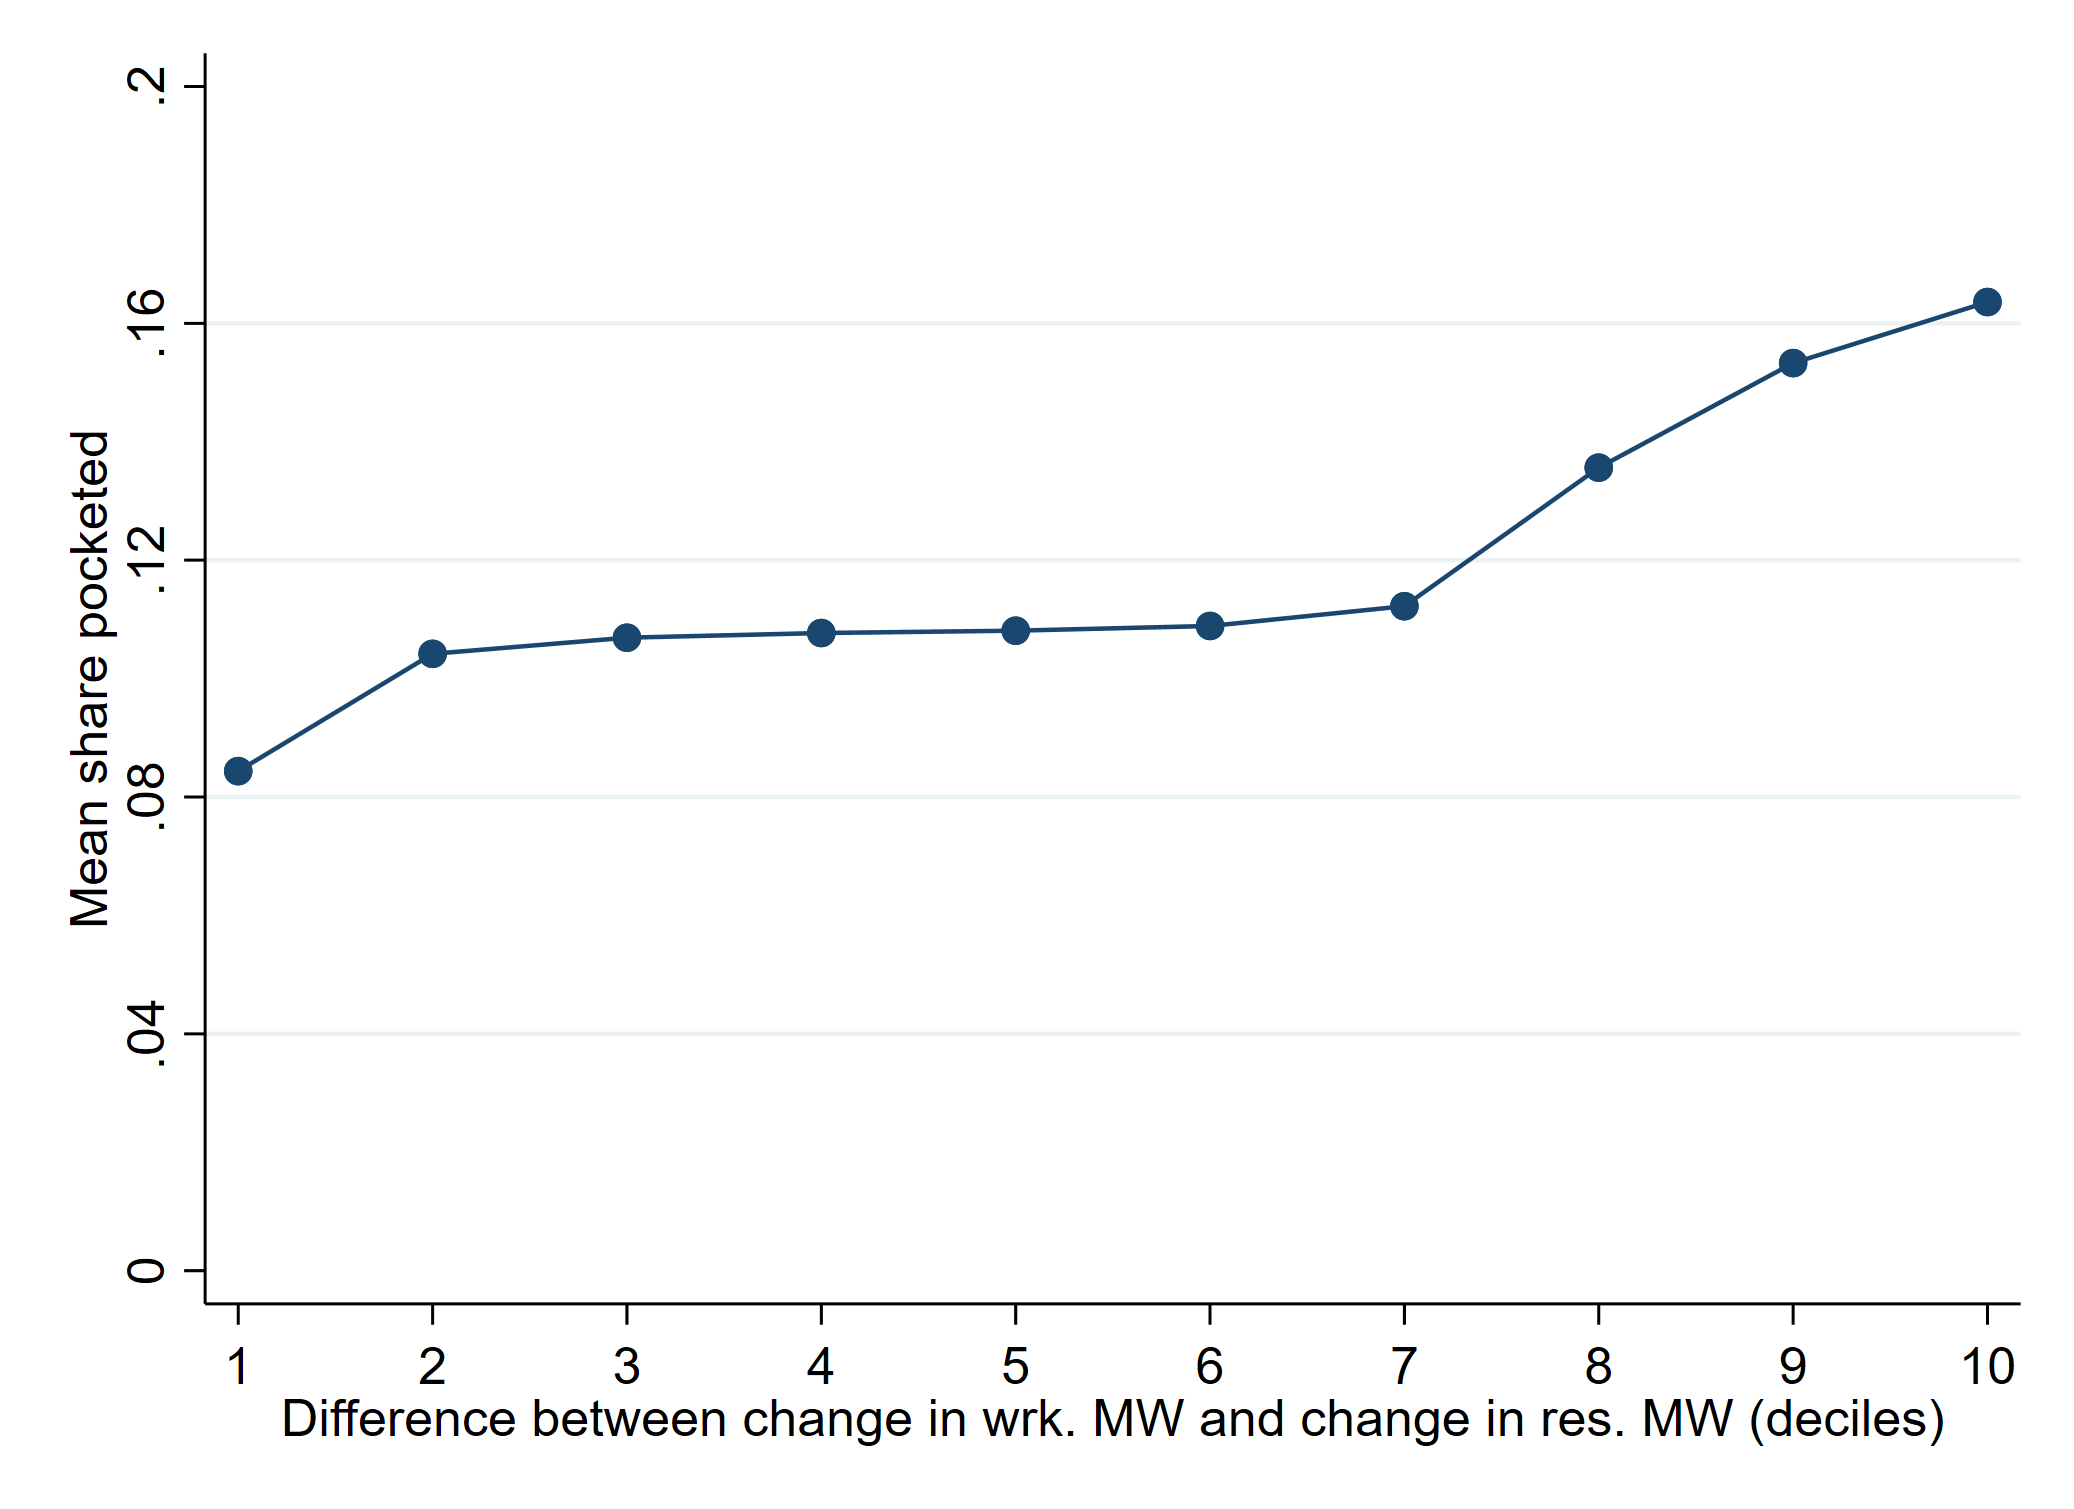
\includegraphics[width = 0.75\textwidth]{counterfactuals/output/deciles_diff.png}

    \begin{minipage}{.95\textwidth} \footnotesize
        \vspace{3mm}
        Notes:
        Data are from the minimum wage panel described in 
        Section \ref{sec:mw_construction} and from LODES.
        The figure shows the average estimate of the shares of the additional 
        income pocketed by landlords $\rho_i$ for each decile of the 
        difference $\Delta \mw_i^{\wkp} - \Delta \mw_i^{\res}$.
        Estimates for lower deciles correspond to ZIP codes where the increase 
        in residence MW was relatively large.
        The unit of observation is the urban ZIP code, where we define a ZIP code 
        as urban if it belongs to a CBSA with at least 80\% of its population 
        classified as urban by the 2010 Census.
        The share pocketed is defined as the ratio between the percent increase 
        in rents and the percent increase in total wages multipled by the share 
        of housing expenditure in the ZIP code.
        To estimate it we follow the procedure described in Section 
        \ref{sec:counterfactual}, assuming the following parameter values: 
        $\beta = 0.0546$, $\gamma = -0.0207$, $\varepsilon = 0.1083$, and 
        $s = 0.35$.
        The figure excludes ZIP codes located in the 60 CBAs for which the average
        estimated change in log total wages was below 0.1\%.
    \end{minipage}
\end{figure}
